% This is a default-selection of plugins that are used widely in this repo.

\documentclass[a4paper,10pt,fleqn]{article}
\usepackage[utf8]{inputenc}

% deutsche Trennmuster etc.
\usepackage[ngerman]{babel}
\usepackage[T1]{fontenc}

% mathematical simbols and fonts
\usepackage{mathtools} 
\usepackage{amssymb}
\usepackage{amsmath}
\usepackage{ntheorem}
\usepackage{polynom}
\usepackage{marvosym}
\usepackage{tabu}
\renewcommand*{\bmod}{\mathbin{\%}}
\everymath{\displaystyle}

\usepackage{multicol}
\usepackage{color}
\usepackage[usenames,dvipsnames]{xcolor}
\setlength{\columnsep}{1cm}
\setlength{\columnseprule}{0.25pt}
\def\columnseprulecolor{\color{gray}}
\usepackage{hyperref}

\usepackage[margin=1.5cm]{geometry}
\usepackage{graphicx}
\usepackage{pgfplots}
\pgfplotsset{compat=1.10}

%Code higlighting

\usepackage{minted}

% make lists more compact:
\newlength{\wideitemsep}
\setlength{\wideitemsep}{.5\itemsep}
\addtolength{\wideitemsep}{-5pt}
\let\olditem\item
\renewcommand{\item}{\setlength{\itemsep}{\wideitemsep}\olditem}
\renewcommand{\arraystretch}{1.25}

\title{Zusammenfassung ExEv}
\author{Fabian Hauser}
 
\begin{document}
\maketitle

\section{Einführung Experimente}

\subsection{Wissenserwerb druch Experimente}
\begin{enumerate}
	\item	Hypothese formulieren
	\item	Daten im Experiment gewinnen
	\item	Hypothese Prüfen
	\item	Gegebenenfalls Modell anpassen
\end{enumerate}

\subsection{Versuchsaspekte}
\begin{itemize}
	\item	Komplexität			(Faktoren, Elemente)
	\item	Kompliziertheit		(Unbekannte oder unverstandene Zusammenhänge, oversimplification)
	\item	Rauschen, Dynamik	(keine Wiederholbarkeit, Zeitliche Variation)
\end{itemize}

\begin{description}
	\item[Validierung] \hfill \\
		Bestätigung des Modells im untersuchten Wertebereich. "Mach ich das richtige?"
	\item[Verifikation] \hfill \\
		Formaler Beweis, dass die Implementation gemäss dem Modell implementiert ist. "Mache ich es richtig?"
\end{description}

\subsection{Prozessmodell}

	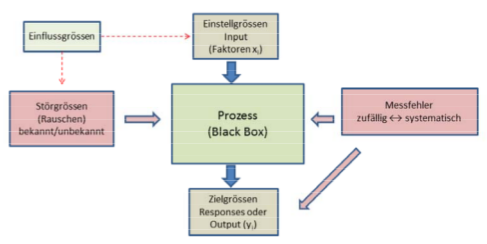
\includegraphics[scale=0.75]{img/prozessmodell.png}

\subsection{Versuchsplanung}

\begin{itemize}
	\item	Zielgrösse / Output
	\item	Einflussgrössen
	\item	Faktoren (vermutete wesentliche Einflussgrössen)
	\item	Faktorenstufen (Werte, die Faktoren in einem Experiment annehmen)
\end{itemize}

\subsection{(Mess-)Fehler}

\begin{description}
	\item[Absolute Fehler] \hfill \\
		Messfehler in einer Masseinheit
	\item[Relative Fehler] \hfill \\
		Fehler in Prozent
	\item[Zufälliger Fehler] \hfill \\
		Fehler, welcher nicht reproduzierbar auftritt
	\item[Systematische Fehler] \hfill \\
		Fehler, welcher Systematisch auftritt (z.B. falsche Lineallänge)
\end{description}


\end{document}